
\Problem{Aparellament màxim en un graf bipartit}

\Statement

Un \textit{graf bipartit} és un graf $G = (U \cup V,\, E)$ on els vèrtexs es
divideixen en dos conjunts disjunts $U$ i $V$ tals que totes les arestes
connecten un vèrtex de $U$ amb un de $V$.

\medskip

Un \textit{aparellament} (\textit{matching}) $M \subseteq E$ és un subconjunt
d'arestes tal que cap parell d'arestes de $M$ comparteixen cap vèrtex. 
La \textit{mida} d'un aparellament és el nombre d'arestes que conté.

\medskip

Un aparellament és un \textit{aparellament màxim} si no existeix
cap altre aparellament de mida més gran.

\medskip
Per exemple, a la figura següent, el primer graf bipartit té un aparellament màxim de 3 arestes que es mostren en negreta i el segon té un aparellament màxim de 5 arestes.

\medskip
\begin{center}
    \begin{latexonly}
        \hspace*{-3cm}
        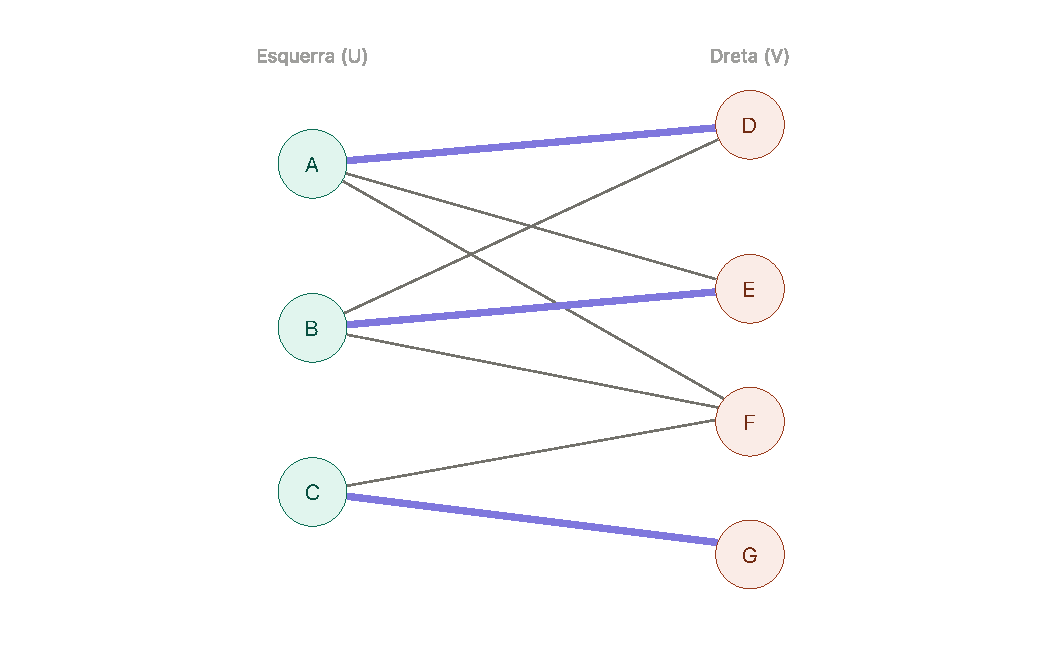
\includegraphics[width=11cm]{exemple1.pdf}
        \hspace*{-4cm}
        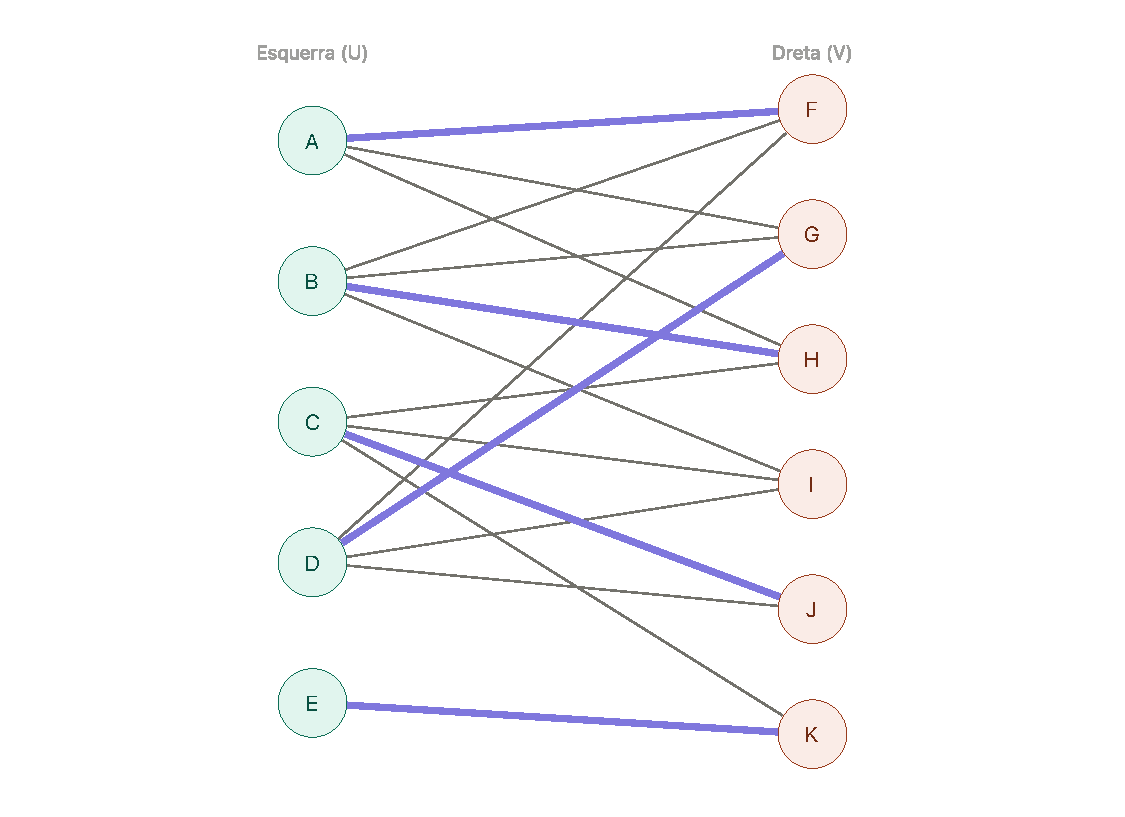
\includegraphics[width=11cm]{exemple2.pdf}
        \hspace*{-3cm}
    \end{latexonly}
    \begin{htmlonly}
        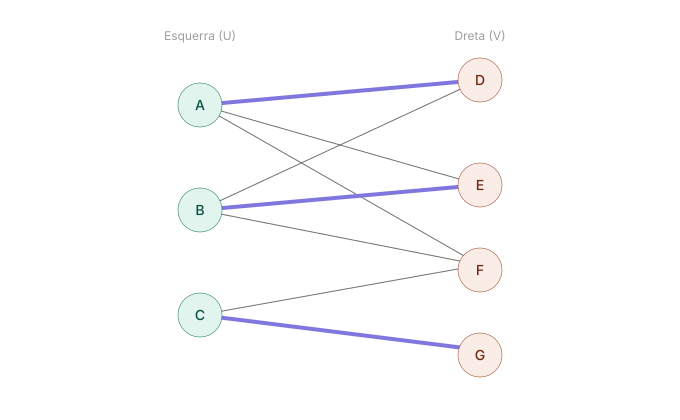
\includegraphics[width=11cm]{exemple1.svg}
        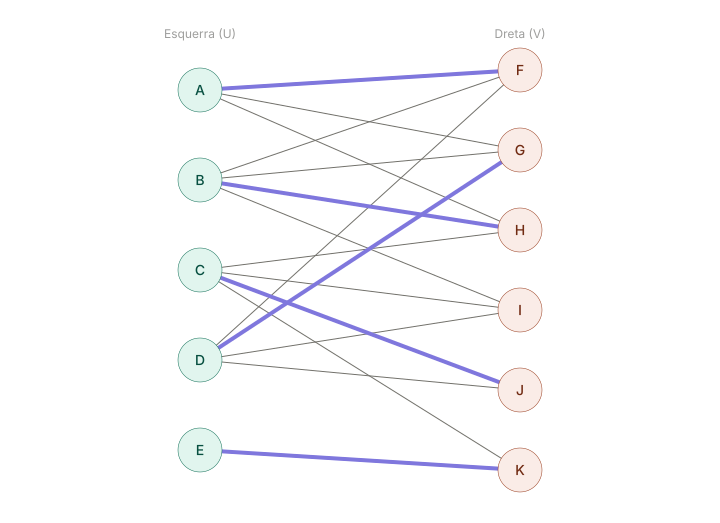
\includegraphics[width=11cm]{exemple2.svg}
    \end{htmlonly}
\end{center}
\medskip

Implementeu un algorisme per trobar la mida d'un aparellament màxim en un graf bipartit. 

\Input

L'entrada consisteix en un graf bipartit descrit per una seqüència d'arestes, cadascuna d'elles descrita per un parell de vèrtexs (paraules) $u$ $v$ de forma que $u \in U$ i $v \in V$.

\Output

La sortida és la mida d'un aparellament màxim del graf bipartit donat.

\subsection*{Codi utilitzable}

Descarregeu-vos el fitxer \textbf{code.py}. Aquest fitxer conté una classe amb la implementació de l'algorisme de Ford-Fulkerson per trobar el flux màxim en una xarxa amb capacitats i un programa principal que l'utilitza.

\SampleTwoCol

